\documentclass{article}
\usepackage[utf8]{inputenc}
\usepackage{emnlp16}
\usepackage{graphicx,hyperref}
\usepackage[table,xcdraw]{xcolor}

\newcommand{\ms}[1]{{\color{cyan}\{\textit{#1}\}$_{ms}$}}

\title{Benchmarking Python Deep Learning Frameworks\\ on Language Modeling }
% feel free to make this title much much better!
\emnlpfinalcopy 

\author{Lucy Lin, George Mulcaire \& Maarten Sap
\\University of Washington}
\date{December 2016}

\begin{document}

\maketitle

\begin{abstract}
Abstraaaact
\end{abstract}


\section{Introduction}
In recent years, deep learning approaches have exploded in popularity due to their performance gains over traditional systems on many tasks. Several deep learning frameworks have been released in response to this, each claiming niche improvements over others, but it is not necessarily clear which frameworks are better suited for which types of applications. Previous comparisons may now be out-of-date (older versions; lack of newer frameworks) or were run against simpler tasks (which might have hidden other interesting performance characteristics).

In this project, we benchmark deep learning frameworks on a complex natural language processing task and rank them based on different performance metrics. Specifically, we look at the following frameworks:
\begin{itemize}
	\item TensorFlow \cite{tensorflow}
	\item Theano \cite{theano}
	\item DyNet \cite{dynet}
\end{itemize}
In natural language processing (NLP), recurrent neural networks (RNNs) are of particular interest because they make use of the sequential nature of language. Benchmarks on RNNs have been run before, but most tasks were benchmarked on toy tasks which do not necessarily reflect performance on real data. For instance, GitHub user \verb!glample!  generated random data to run through their RNN \cite{glample}, which is not realistic. In NLP, we usually turn words into vocabulary-sized one-hot vectors and then embed them (i.e. dimensionality reduction) as hidden-sized vectors. Sparsely learning the embedding matrix, which is usually in the order of $[20,000 \times 200]$, is likely to severely impact performance.


\section{Background}
\subsection{Language Modeling}
The task of language modeling is about estimating probabilities of particular sequences of words. It is used as an invaluable component in various real-world applications such as speech recognition, statistical machine translation, etc. More formally, if $s=\{START,x_1,x_2,...,x_n,STOP\}$ is an n-word sentence, language modelling will try to estimate, for each word $x_i$
its probability given its history: $p(x_i|START,x_1,x_2,...,x_{i-1})$. 
Historically, this task can be done rather simply using an l-th order Markov model, where $p(x_i|START,x_1,x_2,...,x_{i-1}) = p(x_i|x_{i-l},x_{i-l+1},...,x_{i-1})$. However, the Markov assumption does not need to be made with recurrent neural networks, as they have the capabilities to encode much longer histories. With RNNs, we normalize (using softmax) the output of a nonlinear function $f\left(p(x_i|START,x_1,x_2,...,x_{i-1})\right) =softmax\left(f(x_i,START,x_1,x_2,...,x_{i-1})\right)$.

\subsection{Frameworks}
All three frameworks use a symbolic computation graph, which maps operations and variables to nodes in a graph. To perform computation, one has to ``query'' the graph, providing values for variables needed to compute the desired output.
Figure~\ref{fig:compGraph}\footnote{Taken from \cite{tensorflow}} shows an example of a simple computation graph. All three frameworks efficiently handle queries, by only computing nodes that are necessary for the output requested.\ms{Can we confirm that's true?}

\begin{figure}\begin{center}
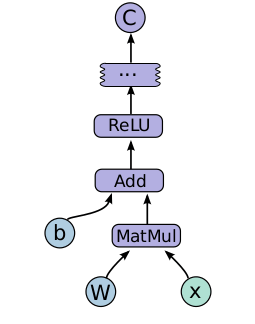
\includegraphics[scale=.4]{graphics/tensorflowGraph.png}
\caption{\label{fig:compGraph}Simple neural computation graph example. \texttt{ReLU} is a rectified linear unit.} 
\end{center}\end{figure}

All our frameworks run a \texttt{Python} wrapper, with a \texttt{C++} backend.
\ms{TODO: more spiel?}
%TensorFlow's computation graph is pure \texttt{Python}, which makes it slower than other frameworks.

\section{Experiments}
\subsection{Data \& Preprocessing}
We chose to focus on the Los Angeles Times subset from 2009 of the GigaWord corpus \cite{gigaword}. Each of these documents is a news article, so we used NLTK’s \cite{nltk} sentence splitter on the articles. Every sentence is then tokenized using NLTK’s \verb!casual_tokenize! function, limiting ourselves to sentences that are $<100$ tokens long. In order to limit overfitting, we replace all words that occurred less than $150$ times by a special \verb!OOV! symbol (this allows the model to be more robust when encountering previously unseen words). We ended up with $1,191,848$ sentences, $27,269,856$ total word tokens and a vocabulary size of $35,642$.

\subsection{Implementation \& Hyperparameters}
Table~\ref{tab:hyperparams} summarizes the hyperparameters chosen for the experiments; there was no cross-validation done since the evaluative performance of the model trained is irrelevant.
\begin{table}\begin{center}
\begin{tabular}{cc}
\textbf{hyperparam} & \textbf{value} \\\hline
RNN type & \texttt{LSTM} \\
hidden size & $256$ \\
optimizer & \texttt{AdamOptimizer} \\
learning rate & $0.003$ \\
batch size & 25 \\
\end{tabular}
\caption{\label{tab:hyperparams}Hyperparameters used in the experiments}
\end{center}\end{table}

Traditionally, neural models are trained until their performance on a \textit{development} set stops improving. Therefore, a full epoch of training (where all the training data is used) is usually followed by a predictive pass through development data.
\section{Benchmarks}
\subsection{Time}
The first benchmark to look at is how long training takes. Table \ref{tab:timing} summarizes various breakdowns.
\begin{table}
\begin{tabular}{c|ccc}
Time & Dynet & TensorFlow & Theano \\ \hline
Convergence & & 35h 25' & \\
Train epoch & & 6h57' &  \\
Test epoch & & 7'45'' & \\
Train batch & & 5'' &  \\
Test batch & & $<$1'' & \\
\end{tabular}
\caption{\label{tab:timing}Total runtime on various subtasks.}
\end{table}

\subsection{Cuda Profiler}
We used the CUDA Profiler Toolkit \cite{nvprof} to characterized our implementations, specifically on a simplified task of training on 1 batch.

We profile which methods take the most amount of time, and look into a variety of metrics.
\begin{itemize}
\item \verb!achieved_occupancy! - fraction of GPU warps used v.s. total number of warps
\item \verb!sm_efficiency! - how much of the runtime is spent performing actual computation
\item \verb!warp_execution_efficiency! - how efficient is execution within a warp; number of registers per thread is a limiting factor.
\item \verb!warp_nonpred_execution_efficiency! - how efficient is execution within a warp on non-predicated (i.e. non-branching) instructions.
\item \verb!dram_read_throughput! - read throughput
\item \verb!dram_write_throughput! - write throughput
\end{itemize}
\section{Discussion}
When looking to use neural network benchmarks, researchers might want to consider various aspects.
\subsection{Programmer Experience}
When adopting new software frameworks, it is important to consider the potential learning curve, as well as higher-level advantages of each framework.

\subsection{TensorFlow}
Pros: easy to use; good support for RNNs and language models; 
Cons: symbolic computation graph is hard to debug; seems slower than others; 
\section{Conclusion}
\section*{Acknowledgments}
We want to thank Emily Furst for helping us with GPU profiling, specifically understanding the CUDA Profiler documentation.
\newpage
\bibliography{references}
\bibliographystyle{emnlp16}
\end{document}
